\chapter{Knowledge Graphs}\label{chap:kgs}

\chapterQuote{\hfill\textit{``To know that we know what we know, and to know that we do not know what we do not know, that is true knowledge.''}}{--- \textit{Nicolaus Copernicus}}

\chapterAbstract{K}{nowledge Graphs (KGs) are a way to structure information by representing them into a series of interconnected facts and relations between them. This chapter gives some context around them. It is divided into the following sections: Section~\ref{sec:kgs-intro} presents a brief history of Knowledge Graphs and their adoption. Section~\ref{sec:kgs-current} goes over some of the more relevant KGs currently. Section~\ref{sec:kgs-applications} goes about some of the many applications KGs are currently being used for. Section~\ref{sec:kgs-challenges} reflects the current open challenges for KGs. Finally, Section~\ref{sec:kgs-summary} summarizes and concludes this chapter.}


\section{Introduction}\label{sec:kgs-intro}
% METER ESTA IDEA AQUI.
% Es gracioso que los grafos de conocimiento al fin y al cabo no representan nada "nuevo" ya que una base de datos relacional puede implementar grafos etc. Se puede mencionar la idea de que los grafos de conocimiento permiten quitar bagaje y tener algo simple de implementar, expandir, y al que aplicar algoritmos.

Before the emergence of knowledge graphs, information was predominantly stored in traditional databases and represented in tabular formats. While these databases were effective at storing structured data, they lacked the capacity to capture the complex relationships and semantics inherent in real-world information.

The concept of knowledge graphs can be traced back to the early days of Artificial Intelligence (AI) research. In the 1960s and 1970s, researchers began exploring methods to represent knowledge in a form that could be understood and utilized by computers. Early endeavors focused on semantic networks, which used nodes to represent concepts and edges to denote relationships between them.

The advent of the World Wide Web in the 1990s brought about an explosion of digital information. As the volume of web content grew, so did the need for more sophisticated methods of organizing and extracting knowledge from this vast repository. This led to the development of the Semantic Web, a vision championed by Sir Tim Berners-Lee, which aimed to make web content machine-understandable.

A pivotal milestone in the evolution of knowledge graphs was the introduction of the Resource Description Framework (RDF) in the late 1990s. RDF provided a standardized way to describe resources on the web and establish links between them. This laid the foundation for the creation of linked data, which allows for the interconnection of disparate datasets on the web.

In 2012, Google introduced the term "Knowledge Graph" as a central element of their search engine. Google's Knowledge Graph aimed to enhance search results by providing contextual information about entities and their relationships. This marked a significant shift towards a more semantically enriched approach to information retrieval.

Rather than a simple collection of relations between names of entities, they started to be seen as a rich, interconnected structure of elements (\textit{``things, not strings''}) with an enormous potential for practical and commercial applications. Many other large companies the likes of Amazon, Facebook, Microsoft and eBay soon followed suit 
% \cite{shrivastava2017, krishnan2018, pittman2017, noy2019},
and the term Knowledge Graph (KG) rose to the popularity it still enjoys nowadays, replacing the denomination ``Knowledge Base''.

Today, knowledge graphs have become a cornerstone of various AI applications, including natural language processing, recommendation systems, and data integration. Their ability to represent complex relationships and semantic context has made them an invaluable tool in the era of big data and advanced machine learning techniques.

% kept this here for the citations...

% Representing and storing structured domain-specific knowledge has been an active research topic since at least 1970, when the first relational databases were introduced \cite{codd1970}. Given their indisputable success, many alternative means of representing knowledge in an structured manner have been proposed over the years. One of such proposals was using what was coined as a \textit{Knowledge Base} (KB) \cite{hayes-roth1983}, a collection of facts that are stored as direct relations between concepts. Contrary to relational databases, which need to go through a normalization process that introduces a number of indirections to represent a piece of knowledge, KBs were considered more straightforward to operate and reason about \cite{russell2020}. A number of Knowledge Bases were thus created and maintained throughout the subsequent years by multiple organizations and research entities, which were both general-purpose~\cite{mahdisoltani2014,lehmann2015dbpedia, rebele2016, carlson2010, bollacker2008, vrandevcic2014} and domain-specific~\cite{chakravarty2017, thorn2013pharmgkb, wishart2009, wishart2008, kanehisa2010}.

% The information inside a Knowledge Base was stored in the form of entities, which represented real-world or domain-specific concepts, and relations that link these entities together. This is known as a triple: a combination of two entities by means of a relation, which usually contains a verb. For example, a KB can represent the fact that Magnus Carlsen is a chess player using the triple \textit{(Magnus Carlsen, plays, Chess)}. Such triples were generally encoded in a KB using the RDF/XML format \cite{decker2000}, or an extension of it called RDFS, which allows for a higher degree of expressivity. However, since RDF/XML is mainly intended for machine use, later KBs also used other formats, like N3, Turtle, or RDF/JSON, which are more human-readable.

% However, the introduction of the Google Knowledge Graph in 2012 \cite{singhal2012} was a pivotal point for both the industrial use and academic research of Knowledge Bases.


% In the following sections, we present the most popular Knowledge Graphs that are under active use today and the ways in which they are constructed. We then discuss the many practical applications that can, and have been, derived from the usage of KGs in commercial and academical contexts. However, despite their many benefits, Knowledge Graphs still present several challenges that must be addressed to improve their functionality and usefulness. Therefore, we also provide an overview of the main open challenges that need to be addressed to refine and improve Knowledge Graphs.

\section{Modern Knowledge Graphs}\label{sec:kgs-current}

% Nowadays, there are a number of popular Knowledge Graphs under active use, either commercial or academical. Some of the most prominent ones are as follows:

\begin{itemize}
    \item \textbf{DBpedia} is a community-driven knowledge graph that extracts structured information from Wikipedia articles. It covers a wide range of topics and provides structured data about entities, their attributes, and relationships. DBpedia utilizes natural language processing and information extraction techniques to parse Wikipedia articles and convert unstructured text into a structured RDF format.
    
    \begin{figure}[!h]
        \centering
        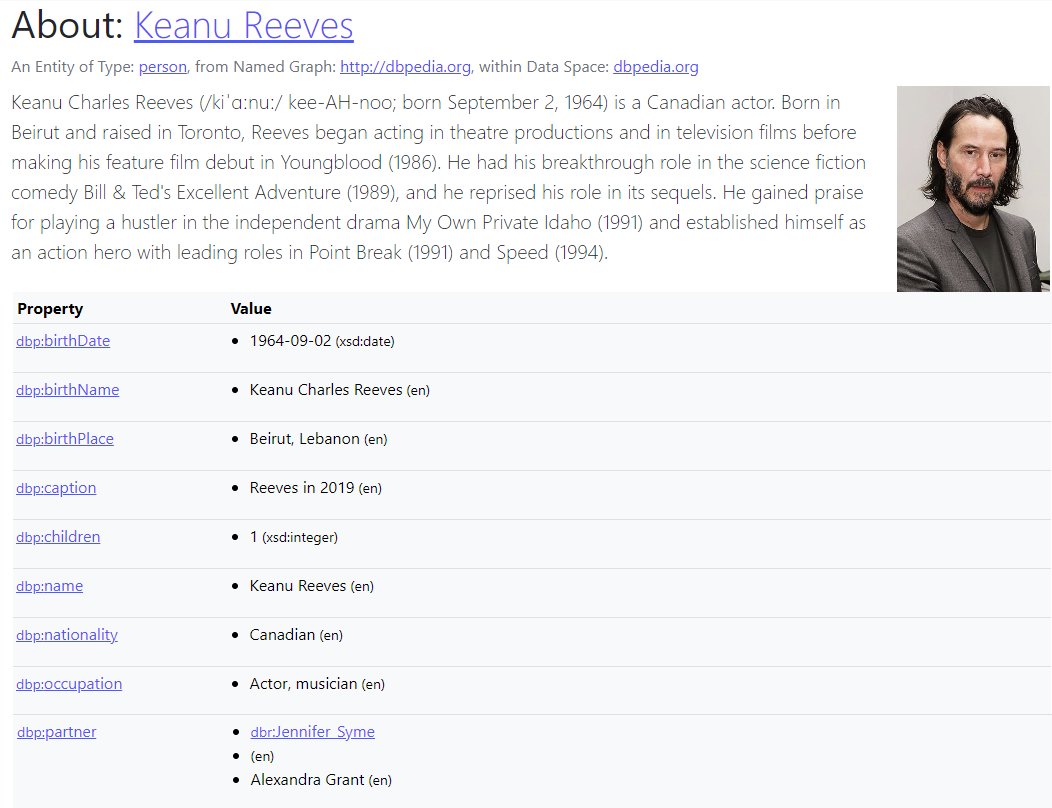
\includegraphics[width=\textwidth]{fig/kgs/Keanu_DBpedia.png}
        \caption{The ontology \textit{Keanu Reeves} in DBpedia}
        \label{fig:kgs-dbpedia}
    \end{figure}
    
    \item \textbf{YAGO} (Yet Another Great Ontology) is a knowledge graph that combines data from Wikipedia, WordNet, and GeoNames. It provides a comprehensive representation of entities and their relationships. Created using automated extraction techniques and ontological alignment to integrate information from multiple sources.
    
    \item \textbf{Wikidata} is a collaborative, multilingual knowledge graph maintained by the Wikimedia Foundation. It serves as a central repository of structured data for Wikimedia projects and beyond, containing information about a diverse set of topics it is built by a global community of volunteers who contribute, edit, and curate data using a web-based user interface.
    
    \begin{figure}[!h]
        \centering
        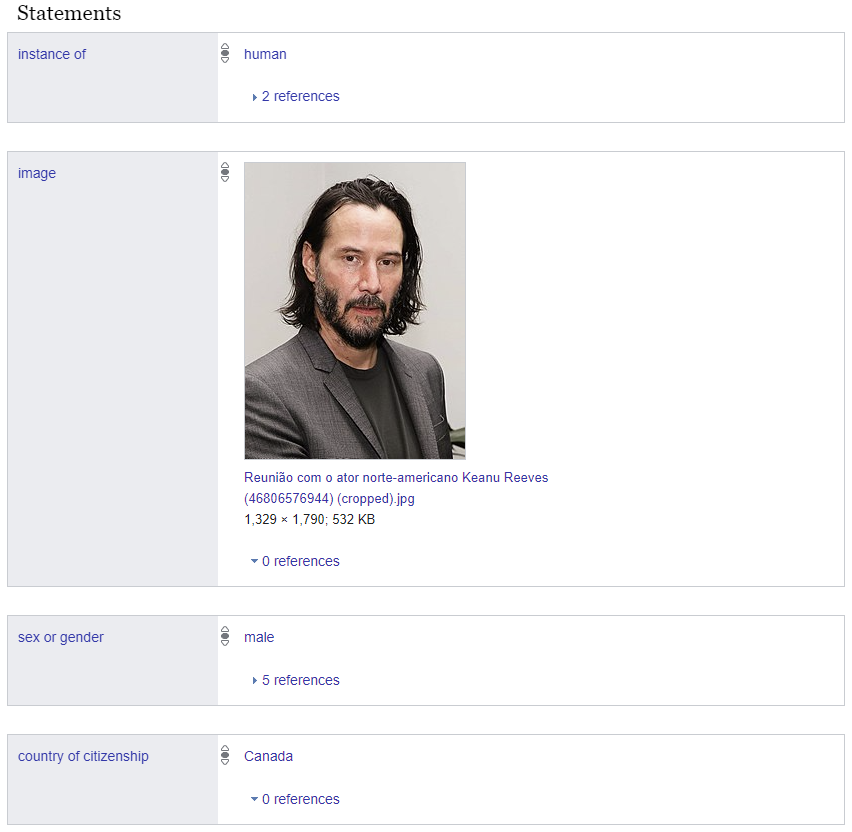
\includegraphics[width=\textwidth]{fig/kgs/Keanu_Wikidata.png}
        \caption{The entity \textit{Keanu Reeves} in Wikidata}
        \label{fig:kgs-wikidata}
    \end{figure}

    % \item \textbf{GeoNames} is a geographical database that provides detailed information about places worldwide, including countries, cities, and landmarks. It also includes coordinates and population data, it combines data from various sources, including official government databases, with user contributions and validation processes.

    \item \textbf{UMLS (Unified Medical Language System)} is a comprehensive ontology and knowledge graph for the biomedical domain. It integrates terminology and data from various biomedical sources. UMLS is built through a combination of manual curation by domain experts and automated processes for integrating and mapping different terminologies.
    
    \item \textbf{Freebase (Now Part of Wikidata)} was a large-scale knowledge graph acquired by Google in 2010 and later integrated into Wikidata. It contained structured data on a wide array of topics, including people, places, and concepts. It was constructed through a combination of automated data extraction, crowd-sourcing, and expert curation.
    
    \item \textbf{WordNet} is a lexical database of the English language, organized in a semantic network. It groups English words into sets of synonyms (synsets) and provides short, general definitions. WordNet is manually constructed by lexicographers who define word meanings and establish semantic relationships between words.
    
    \item \textbf{NELL (Never-Ending Language Learning)} is a project aimed at creating a machine learning system that continuously learns to extract structured information from the web. It aims to discover new facts about entities over time it uses a combination of natural language processing, machine learning, and information extraction techniques to learn and update its knowledge base.
\end{itemize}

\section{Applications}\label{sec:kgs-applications}

Knowledge graphs, as we explored in the preceding chapter, are structured representations of information that emphasize the interconnectedness of entities, attributes, and relationships. This section delves into the practical applications and diverse utility of knowledge graphs across a spectrum of domains. The power of knowledge graphs lies not only in their capacity to organize information but also in their ability to unlock a deeper layer of context, semantics, and relationships within data. 

They have emerged as a foundational tool in modern information processing and artificial intelligence. In this chapter, we delve into the diverse and powerful applications of knowledge graphs across various domains. From enhancing search engines to revolutionizing recommendation systems, knowledge graphs play a pivotal role in extracting valuable insights and enabling intelligent decision-making.

This chapter explores five prominent applications of knowledge graphs, each showcasing their versatility and impact in different realms of information processing, such as information retrieval, data analysis, and decision support. We illustrate how knowledge graphs have transformed traditional approaches, enabling more accurate, contextually aware, and personalized interactions with data.

\begin{itemize}
    \item \textbf{Semantic Search and Information Retrieval}:
    Knowledge Graphs provide a structured foundation for deducing the context between entities by understanding the intricate relationships between them. Unlike traditional keyword-based searches, semantic search engines, empowered by knowledge graphs, consider the deeper meaning and connections within the data, they ensure that search results are more accurate and contextually meaningful. This is especially crucial in fields like healthcare, legal research, and scientific studies where precision in information retrieval is essential. Through semantic search, users can navigate complex datasets with greater precision, uncovering insights that might be missed in traditional keyword-based searches.

    For instance, in a healthcare knowledge graph, the relationships between symptoms, diagnoses, and treatments allow for more precise and contextually relevant search results. This is vital in scenarios where accuracy and depth of information retrieval are paramount.

    
    \item \textbf{Recommendation Systems}:
    Knowledge graphs play a pivotal role in recommendation systems, revolutionizing how personalized suggestions are generated. Recommendation systems, at their core, rely on understanding user behavior and preferences. Knowledge graphs provide the structured foundation needed to model these relationships effectively. By incorporating nuanced connections, recommendation systems can go beyond surface-level patterns, uncovering unexpected associations that lead to more meaningful and relevant suggestions. By modeling rich semantic connections between users, items, and their attributes, knowledge graphs enhance the accuracy and relevance of recommendations. 
    
    This is particularly crucial in domains like content streaming platforms, e-commerce, and content curation, where tailoring suggestions to individual tastes can significantly enhance the user experience. Knowledge Graphs elevate the accuracy and effectiveness of recommendation engines. This results in more engaged users, higher conversion rates, and ultimately, a more satisfying user experience.

    \item \textbf{Natural Language Processing (NLP)}:
    Knowledge graphs provide a structured framework for representing and understanding textual information which significantly enhances natural language processing (NLP) tasks. It allows for more accurate and nuanced language understanding, leading to improved tasks such as entity recognition, relationship extraction, and question-answering.

    By incorporating semantic relationships between entities and their attributes, knowledge graphs enrich language understanding. They serve as a fundamental tool for NLP applications. They allow for a more nuanced analysis of textual data by considering not just individual words, but also their relationships within a broader context. Knowledge graphs enable NLP systems to go beyond basic language processing, enabling them to grasp the complexities of human communication more effectively.
   

    \item \textbf{Contextual Analysis and Decision Support}:
    Contextual analysis involves examining information within the broader framework of its surroundings, considering the environment, relationships, and relevant circumstances that influence its meaning or interpretation. It is crucial to understand the full significance of data. It helps in avoiding misinterpretations that can occur when information is considered in isolation. By taking into account the surrounding context, analysts can gain deeper insights and make more informed decisions. 
    
    Knowledge graphs enhance contextual analysis by providing a structured framework for representing relationships and contextual information between entities. These graphs incorporate temporal, hierarchical, and semantic dimensions, allowing for a comprehensive understanding of data within its broader context. Moreover, knowledge graphs facilitate context-aware queries, enabling users to retrieve information based on specific contextual constraints. This not only supports decision-making but also empowers analysts to uncover hidden patterns and dependencies within the data, ultimately leading to more informed and effective analyses.

    \item \textbf{healthcare}:
    In healthcare, knowledge graphs serve as a powerful tool for representing, organizing, and analyzing complex medical information. They provide a structured framework that captures relationships between medical entities, their attributes, and contextual information. For instance, a healthcare knowledge graph can model the relationships between symptoms, diagnoses, treatments, medications, and patient histories. This enables comprehensive and contextually rich representations of medical data, which is crucial for accurate diagnosis, treatment planning, and research.

    One of the key strengths of knowledge graphs in healthcare lies in their ability to integrate diverse sources of medical information. They can incorporate data from electronic health records (EHRs), medical literature, clinical trials, and other healthcare databases. This integration enables a holistic view of a patient's medical history and facilitates evidence-based decision-making by healthcare professionals.
    
    Furthermore, knowledge graphs support clinical decision support systems (CDSS) by providing a structured foundation for generating patient-specific recommendations and alerts. For example, a CDSS built on a healthcare knowledge graph can analyze a patient's symptoms, medical history, and medication interactions to offer tailored treatment suggestions. This not only enhances the quality of care but also helps healthcare providers stay up-to-date with the latest medical knowledge.
    
    In addition, knowledge graphs are invaluable for medical research and innovation. They enable researchers to explore relationships between genetic factors, diseases, treatments, and outcomes. This can lead to discoveries about disease mechanisms, personalized medicine approaches, and the development of new therapies.
    
\end{itemize}

\section{Open challenges}\label{sec:kgs-challenges}
While knowledge graphs offer a powerful framework for organizing and leveraging structured data, they are not without their complexities and hurdles. In this section, we turn our attention to the open challenges that persist in the field of knowledge graphs. These challenges encompass three critical domains: integration, completion, and reasoning. Addressing these issues is essential for unlocking the full potential of knowledge graphs in diverse applications. Let's delve into each of these challenges and explore the research frontiers that seek to overcome them.

\subsection{Integration - Joining diverse data sources}
Knowledge graph integration addresses the crucial task of amalgamating information from disparate sources into a unified, coherent representation. This process is instrumental in creating comprehensive knowledge graphs that encapsulate a wide array of domains. Ontology-based integration employs predefined schemas to structure data, ensuring compatibility across diverse sources. Federated approaches, on the other hand, enable querying across distributed databases, extracting relevant information from each source. Schema matching and alignment techniques aim to identify correspondences between different schemas, facilitating the mapping of data elements.

These approaches collectively form the bedrock of knowledge graph integration, enabling the creation of holistic, interconnected representations. Integration is particularly challenging when dealing with multilingual data, as language nuances add an additional layer of complexity. The global nature of information demands knowledge graphs that transcend language barriers. Multilingual knowledge graphs integrate data from various linguistic sources, enabling a truly global perspective. Machine translation techniques play a pivotal role, in facilitating the transformation of content between languages. Additionally, cross-lingual entity linking ensures that entities mentioned in different languages are correctly aligned, enhancing the coherence and richness of the knowledge graph.

Ambiguity in entity references poses a significant challenge in knowledge graph integration. Entity disambiguation techniques strive to resolve this ambiguity by identifying and linking mentions of the same entity across different data sources. Methods based on contextual information, entity co-occurrence, and semantic similarity have shown promise in disambiguating entities accurately.

\subsection{Completion - Finding missing information}

Knowledge graphs are prone to incompleteness due to the inherent challenges in capturing all facets of real-world information. Incomplete knowledge graphs often arise from limitations in data collection, varying levels of detail in different domains, or evolving sources of information. 

Additionally, semantic gaps may emerge when attempting to represent complex relationships or when dealing with ambiguous entities. Knowledge graph completion plays a vital role in mitigating these shortcomings in order to refine the graph's structure to empower applications, by providing a more comprehensive and accurate representation of the underlying domain.

Knowledge graph completion is the task of predicting missing or incomplete information within a knowledge graph it is an indispensable task in enhancing their comprehensiveness and usability. The process of completion involves inferring new relationships or attributes for existing entities, ultimately enriching the graph's representation. By predicting these missing links, knowledge graph completion enables more accurate querying, reasoning, and recommendation within the graph. 

Knowledge graph completion is executed through a variety of techniques, each designed to infer missing relationships or attributes within the graph. These approaches leverage the existing structure of the knowledge graph, exploiting patterns and dependencies to make accurate predictions. One common strategy involves embedding-based models, which represent entities and relationships as vectors in a continuous space. These models aim to learn embeddings that capture the underlying semantics of the graph, allowing for the extrapolation of missing information. Additionally, rule-based methods utilize logical rules to deduce new relationships based on existing ones. These rules can be hand-crafted or learned from the data, providing a structured approach to completion.

Another prevalent approach in knowledge graph completion involves utilizing graph neural networks (GNNs). These specialized neural networks operate directly on the graph structure, enabling the propagation of information through nodes and edges. By leveraging the local and global connectivity patterns, GNNs can uncover complex dependencies and infer missing links effectively. Additionally, path-based techniques explore sequences of relationships within the graph to identify latent connections between entities. These methods analyze the paths connecting entities and use them to make predictions about missing links.

Once the new information has been inferred it can be used to enrich the KG by adding the missing triples obtained from this process back into the KG. This completion task can be performed every time the KG is extended due to temporal shifts in the information it holds, this way the KG will always be up to date.

\subsection{Reasoning - extracting deeper insights}

In regard to knowledge reasoning, different nomenclatures have been incepted in academic circles. Initially, Reasoning is the process of analyzing, synthesizing and deciding on several matters, it begins with collecting data in the form of facts and discovering interrelationships between them to then develop new insight, In short, reasoning is the process of "drawing conclusions from existing facts by the rules"\cite{sutton2018reinforcement}.

Reasoning techniques developed and so did its description, including the capacity to understand things, apply logic, and validate elements based on existing knowledge. In other words, the mechanism behind inferring new knowledge is based on the existing facts and logical rules. In general, knowledge reasoning is defined as the process of using known knowledge to infer new knowledge.

The internet made available for dataset sizes to explode in size so traditional methods could not adapt to the amount of data generated. For this reason, data-driven machine reasoning methods have gradually become the mainstream of knowledge reasoning research. With the development of knowledge graphs, reasoning over them has gained traction in research.

Its goal is to use machine learning methods to infer potential relations between entity pairs and identify erroneous knowledge based on existing data automatically with the purpose of complementing KGs while obtaining logical rules to accompany the knowledge generated.

% Knowledge reasoning based on logic rules 
% Knowledge reasoning based on distributed representation (Knowledge reasoning based on tensor factorization)

% Knowledge reasoning based on neural network
% (Knowledge reasoning based on recurrent neural network)
% (Knowledge reasoning based on reinforcement learning)

% application of KG reasoning:

Several KG reasoning techniques exist, Inference techniques can perform domain knowledge reasoning through modeling domain knowledge and rules, which can support automatic decision-making, data mining and link prediction. It is performed by applying logical rules and algorithms to traverse, analyze, and connect entities and relationships within the knowledge graph. These rules encode domain-specific knowledge and can be hand-crafted or learned from data.

Embedding-based reasoning leverages continuous vector representations of entities and relationships to perform operations that approximate logical reasoning. Graph neural networks (GNNs) \cite{sola2022} are a powerful approach that directly operates on the graph structure, enabling the propagation of information and capturing complex dependencies.

% \todo{Figure on KG reasoning process...}

Knowledge graph reasoning offers significant improvements over simple completion tasks. While completion focuses on predicting missing links or attributes, reasoning enables a deeper level of understanding by inferring complex relationships and uncovering latent patterns. It goes beyond the immediate graph structure to extract higher-order knowledge, making it invaluable in tasks that require sophisticated analysis and decision-making.

Our approach, SpaceRL, places a particular emphasis on knowledge graph reasoning. By incorporating reinforcement learning techniques, we aim to enhance the reasoning capabilities of agents navigating knowledge graphs. This allows for dynamic exploration and exploitation of the graph's structure, leading to more effective inferences and insights. In future explorations, we intend to delve deeper into this critical aspect, refining and extending SpaceRL to unlock even greater potential in knowledge graph reasoning.

\section{Summary}\label{sec:kgs-summary}
This chapter serves as an introduction to Knowledge Graphs, and initiates the reader with a portrayal of their historical evolution and fundamental attributes. Additionally, it offers a comprehensive overview of noteworthy Knowledge Graphs currently prevalent. The discourse extends to an exploration of pragmatic applications emanating from Knowledge Graphs, elucidating their pervasive influence on our daily activities. Concluding this exposition, the chapter scrutinizes enduring challenges inherent in the domain of Knowledge Graphs, specifically focusing on unresolved issues such as integration, completion and reasoning.